\documentclass[11pt]{article}
%\usepackage{endfloat}
\usepackage[paperwidth=8.5in,paperheight=11in,margin=1in]{geometry}
\usepackage{xr}
\usepackage{amsmath}
\externaldocument{paper}
%% HACKS %%
 
% For section headers starting with S
\renewcommand{\thesection}{S.\arabic{section}}
\renewcommand{\thesubsection}{\thesection.\arabic{subsection}}
 
% Hack for making SOM Equations Conform to Science Format
%
% e.g. (S1), (S2), etc
% Requires AMS
\makeatletter %% With ams
\def\tagform@#1{\maketag@@@{(S\ignorespaces#1\unskip\@@italiccorr)}}
\makeatother
 
% Hack for making figures Say \figurename S\thefigure, e.g. Figure S1:
%\makeatletter
%\makeatletter \renewcommand{\fnum@figure}
%{\figurename~S\thefigure}
%\makeatother
 
% use bibnumfmt to change style at the end of the document
%\renewcommand{\bibnumfmt}[1]{[S#1]}
% citenumfont command adds S to all numbers
%\newcommand{\citenumfont}[1]{\textit{S#1}}
 
\newcommand{\myfigurename}{Figure}
\newcommand{\myref}[1]{\ref{#1}}
\newcommand{\suppref}[1]{S\ref{#1}}
\newcommand{\suppfigurename}{Figure}
 
\usepackage{tikz}
\usepackage{amsmath,amssymb}
\usetikzlibrary{automata, arrows, positioning, shapes, snakes}
 
\newcommand{\row}[2]{\ensuremath{#1_{#2 \cdot}}}
\newcommand{\col}[2]{\ensuremath{#1_{\cdot #2}}}
\DeclareMathOperator{\EX}{\mathrm{E}}% expected value
\DeclareMathOperator{\Var}{\mathrm{Var}} 
\DeclareMathOperator{\Cov}{\mathrm{Cov}} 


%END HACKS

\usepackage{graphicx}

\title{Supporting Information}
\author{}
\begin{document}

%We want to assay every site in the genome
%Accurate whole genome sequencing is too expensive
%SNP arrays and low-pass sequencing are therefore the most used
%technologies
%They have different strengths and weaknesses
%A principled integration framework might improve calling


\maketitle

\section{Methods}

\subsection{The PIGEAN model}

Given a trait (which may be either a quantitative trait or liability
for disease), we assume that each gene $i\ldots
N$ either is or is not involved in the trait, indicated as $d_i=1$ and
$d_i=0$ respectively. We refer to genes with $d_i=1$ as
trait-relevant (or disease-relevant); these can be interpreted as genes that can be
perturbed in a human (i.e. via a compound or editing of the
gene sequence) and result in an altered value for the trait. This binary notion of trait-relevance is
a simplification of reality and does not capture the notion that some
genes may permit perturbations that cause larger effects on the trait
than other genes.

By definition, trait-relevant genes are a superset of the genes for which genetic
variants will exhibit association with the trait. However, many
trait-relevant genes will not have variants with reported
associations, due to either (a) insufficient power of current datasets
to detect association between the trait and a variant that impacts the
gene's coding sequence or regulation; or (b) a lack of variants in
the population (either due to evolutionary forces or luck) that
perturb the gene in a manner that affects the trait. Therefore,
although our goal is
ultimately to elucidate the full set of genes relevant to the trait, human genetics will produce an incomplete list due to
either transient data limitations or fundamental population limitations.

We use $\mathcal{D}_i$ to refer to association data for gene
$i$. We consider four types of association data:
\begin{itemize}
  \item GWAS association data consists of common variants linked to
    the gene and their summary statistics (p-values, effect sizes, and
    standard errors). GWAS summary statistics can be downloaded from
    resources such as the GWAS catalog\cite{} or the Association to Function
    Knowledge Portal\cite{}.
  \item ``Known'' disease gene lists consist of a set of genes previously
    established as harboring variants that influence the trait, together with a confidence level (represented as a
    probability) that the gene is in fact relevant to the rare
    disease. Disease gene lists for rare diseases are available (with confidence
    levels) from resources such as Orphanet\cite{} or the GenCC\cite{}, while gene
    lists for complex traits are available from resources such as
    the Human Phenotype Ontology\cite{}.
  \item Rare disease exome sequence data consists of case and control
    variant counts and frequencies, together with annotations of
    variant deleteriousness (i.e. from REVEL\cite{},
    AlphaMissense\cite{}, or LofTee\cite{}). 
  \item Complex trait exome sequence data consists of gene-level
    summary statistics (p-values, effect sizes, and standard errors),
    obtained from burden tests across one or more masks and collapsed
    into a single aggregate score for each gene.
\end{itemize}
In the current manuscript, we focus only on GWAS association data and
known disease gene lists, but we derive equations for all four cases below.

We define the ``direct genetic support'' of a gene as
$\Pr\left(d_i|\mathcal{D}_i\right)$ -- that is, the probability that
the gene is trait-relevant conditional upon the association data
observed for it. If multiple types of genetic association data is
available for the gene, then the direct genetic support is conditional
upon all types of association data; i.e. we can explicitly define
\[\Pr\left(d_i|\mathcal{D}_i\right) =
\Pr\left(d_i|\mathcal{D}^g_i,\mathcal{D}^k_i,\mathcal{D}^c_i,\mathcal{D}^e_i\right)\]
where $\mathcal{D}^g_i$, $\mathcal{D}^k_i$, $\mathcal{D}^c_i$, and
$\mathcal{D}^e_i$ are GWAS, known genes, rare disease exome sequencing counts, and
complex trait exome gene-level associations.

We define the ``indirect genetic support'' of a gene as
$\Pr\left(d_i|\mathcal{D}_{-i}\right)$, where $\mathcal{D}_{-i} :=
\left\{\mathcal{D}_k : k \neq i\right\}$ -- that is, the probability that
the gene is trait-relevant conditional upon the association data
observed for all genes other than $i$ (for GWAS association data, it
is possible that association data for genes $i$ and $k$ may share
SNPs in common if the genes are nearby each other and SNPs have
probabilities of being linked to multiple genes). The indirect genetic
support of a gene combines with its direct support to produce its
combined support, or $\Pr\left(d_i|\mathcal{D}_{i},\mathcal{D}_{-i}\right)=\Pr\left(d_i|\mathcal{D}\right)$
The intuition as to
why association data for gene $k$ can influence the genetic support
for gene $i$ is if the two genes are in a common biological process
-- if the process is relevant to the trait, as demonstrated by an
association observed for variants of gene $k$, then it increases the
probability that other genes in the process are also relevant to the
trait. Although it is not necessary for the subsequent derivation, it
a biological process can be thought of mathematically as a (sparse)
function that maps genes to probabilities of membership in the
process; or, equivalently, a set of genes annotated with their
probability of membership in the process.

We do not observe biological processes (in the language of machine
learning, they are ``latent'' structures), but there are many
experimental or \textit{ad hoc} approaches that produce noisy readouts of
processes. For example,
\begin{itemize}
  \item databases such as Reactome\cite{},
Wiki processes\cite{}, or the Gene Ontology\cite{} represent curated
knowledge of biological pathways and gene functional categories
  \item genes whose expression is up or down regulated in response to a cellular stimulus
    are more likely to participate in a common process
  \item genes whose alteration causes a similar animal model phenotype
    are more likely to participate in a common process
  \item genes that co-occur in the literature with a biological
    concept (or term) are more likely to participate in a common process
\end{itemize}
These readouts can be modeled as gene ``functional annotations'' --
that is, any numerical value that can be assigned to genes. An
important special case of a functional annotation is a gene set --
this is the case when genes are assigned either values of zero or
one. However, a functional annotation is a more general term and can
encompass values such as expression levels in a tissue or co-occurrence
weights with a literature term. There are millions of functional
annotations available for genes\cite{}, from varying sources and of
varying quality. Scientists use functional annotations constantly and often
implicitly to prioritize genes for further study. The challenge is
that with so functional annotations available, it is unclear which
ones are most predictive of trait-relevant processes, the degree to
which they predict trait-relevant processes, and the extent to which
they are additive as opposed to redundant.

We model the degree to which each annotation predicts trait-relevance
through the following equations:
\[ d_i \sim \text{Bern}\left(y_i\right) \]
\[ \log(\frac{y_i}{1-y_i}) = \sum_jX_{ij}\beta_j + \alpha_i +
\log\left(\frac{\pi}{1-\pi}\right) \]
\[ \beta_j \sim \delta_j{\mathcal N}\left(0, \sigma_j^2\right) \]
\[ \alpha_i = \alpha \sum_jX_{ij}\]
\[ \sigma_j^2 = \sigma^2 \mathrm{sd}_i\left(X_{ij}\right)^{w}\]
\[ \delta_j \sim \text{Bern}(p) \]
Where $X_{ij}$ for $j=1\ldots M$ is the value of annotation $j$ for gene $g_i$, $\beta_j$
is the ``effect size'' of annotation $j$ on the gene's (log-odds)
probability of disease relevance, $\pi$ is the background (or average) probability
of disease relevance, and $\alpha$, $\sigma$, $p$, and $w$
are regularization parameters. Note that the $d_i$ and $\beta_j$
values are latent, while the $X_{ij}$ values are fully observed.

A graphical model of these random variables is shown in Figure \ref{graphical_model}.

\begin{figure}[ht]
\begin{center}
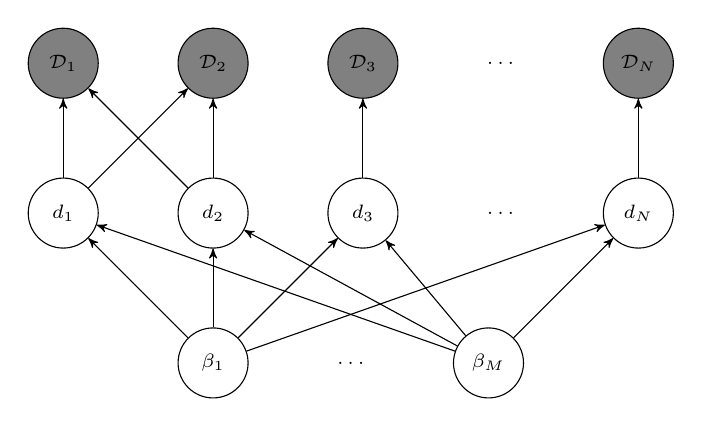
\begin{tikzpicture}[>=stealth',auto, font=\scriptsize]
  \tikzset{ellipse/.style={draw,ellipse}}

  \tikzset{
    blank/.style={
      text centered},
    circ/.style={
      circle,
      draw=black,
      minimum height=.35in,
      text centered},
    obs/.style={
      circle,
      draw=black,
      fill=gray,
      minimum height=.35in,
      text centered}}

  \node[obs] (to1) {$\mathcal{D}_1$};
  \node[obs] (to2) [right=of to1] {$\mathcal{D}_2$};
  \node[obs] (to3) [right=of to2] {$\mathcal{D}_3$};
  \node[blank] (tospace) [right=of to3] {$\ldots$};  
  \node[obs] (ton) [right=of tospace] {$\mathcal{D}_N$};
  \node[circ] (t1) [below=of to1] {$d_1$};
  \node[circ] (t2) [below=of to2] {$d_2$};
  \node[circ] (t3) [below=of to3] {$d_3$};
  \node[blank] (tspace) [right=of t3] {$\ldots$};  
  \node[circ] (tn) [below=of ton] {$d_N$};
  \node[circ] (e1) [below=of t2] {$\beta_1$};
  \node[blank] (espace) [right=of e1] {$\ldots$};  
  \node[circ] (em) [right=of espace] {$\beta_M$};

  \path[->] (e1) edge (t1);
  \path[->] (e1) edge (t2);
  \path[->] (e1) edge (t3);
  \path[->] (e1) edge (tn);
  \path[->] (em) edge (t1);
  \path[->] (em) edge (t2);
  \path[->] (em) edge (t3);
  \path[->] (em) edge (tn);

  \path[->] (t1) edge (to1);
  \path[->] (t2) edge (to2);
  \path[->] (t3) edge (to3);
  \path[->] (tn) edge (ton);

  \path[->] (t1) edge (to2);
  \path[->] (t2) edge (to1);

\end{tikzpicture}
\end{center}
\label{graphical_model}
\end{figure}



The regularization parameters control model sparsity and
over-fitting. Specifically:
\begin{itemize}
  \item We impose a ``spike and slab'' prior on the $\beta_j$ values,
    which asserts that (a) most annotations have zero effect on a
    gene's trait-relevance and (b) those that do have effects on the
    (log-odds) of trait-relevance that are normally distributed. The
    parameter $p$ controls the probability that the effect is
    non-zero, and the $\sigma_j$ parameter controls the variance of
    the conditional effect size distribution
  \item We use an annotation specific variance $\sigma_j$ related to
    a power $w$ of the variance of the gene annotation (across
    genes). Intuitively, ``larger'' or more profligate annotations
    (i.e. those with more genes having non-zero values)
    should have lower power to predict trait-relevance, since they are
    less specific biologically. Traditional gene set enrichment approaches
    implicitly assume that $w=0$, which biases results toward larger gene sets,
    as those have smaller standard errors. A value of $w=-2$ adjusts
    for this bias, and is commonly used in the mathematically similar
    scenario of modeling SNP effect sizes\cite{}.
    \item Analogous to the $w$ parameter, we use an $\alpha$ parameter
      to control biases in favor of genes with more annotations. For
      reasons discussed below\ref{}, genetic support is biased toward
      positive values, and therefore genes with more annotations
      (i.e. better studied genes) typically have higher support unless
      this is controlled for. We typically set $\alpha$ (i.e. via
      linear regression)
      such that there is no relationship between a gene's size and its
      $d_i$ value.
\end{itemize}

\subsection{Fitting the model}

Because the $d_i$ and $\beta_j$ values are latent, we must infer them
from the observed association data $\mathcal{D}$ across all
genes. Specifically, we want to infer the joint distribution
\[\Pr\left(d,\beta|\mathcal{D}\right)\]
Analytically determining an equation for this distribution is intractable, and therefore
we use Gibbs sampling to sample from the joint distribution. Gibbs
sampling proceeds by iteratively drawing samples from the
distribution of each variable conditional upon the current samples for
all other variables. In our case, we have $N$ variables $d_i$ and $M$
variables $\beta_j$. A basic Gibbs sampler would 
need to derive and sample from the conditional distributions
\[\Pr\left(d_i|\mathcal{D},d_{-i},\beta\right)\]
\[\Pr\left(\beta_j|d,\mathcal{D},\beta_{-j}\right)\]
Instead, we employ a more efficient form of Gibbs sampling, termed
block Gibbs sampling, that iterates between sampling all $d$ values
and all $\beta$ values simultaneously:
\[\Pr\left(d|\mathcal{D},\beta\right)\]
\[\Pr\left(\beta|d,\mathcal{D}\right)=\Pr\left(\beta|d\right)\]
The right hand side of the second equation follow from the
conditional dependencies encoded in our model, implying that we
can ignore association data when sampling from the distribution for
$\beta$ if the $d$ values are observed, as in this case the
association data adds no additional information.

Sampling from $\Pr\left(\beta|d\right)$ is itself non-trivial. The
equations for the posterior distribution of variables with spike and slab
priors has previously been studied in the context of polygenic risk
scores -- specifically, the LD-pred method\cite{}. In this work, the
true effect sizes of SNPs on a quantitative trait have a spike and
slab prior, they affect the trait additively, and the observed data is
the marginal estimates of the SNP effect sizes from a series of
univariate regressions of observed trait values (in individuals) and
the value (0, 1, or 2) of the SNP. Furthermore, the equations used to
derive the posterior estimates of SNP effect sizes in this setting
have been shown to apply to binary traits as well, provided the
marginal SNP effect sizes are expressed in units of $\log(OR)$\cite{}, which
holds if they are obtained from a logistic regression of individual
disease status on SNP value. In our setting, the equations relating
annotation effect sizes $\beta_j$ to gene trait-relevance $d_i$ are
identical to those relating SNP effect sizes to individual disease
status (intuitively, annotations correspond to SNPs and genes
correspond to individuals). Therefore, we can follow the same
procedure used by LD-pred\cite{} to sample from the joint distribution
of $\beta$ values. 

Practically, this entails (a) running a univarate logistic regression of $d$ on each
    $\beta_j$ to obtain marginal annotation effect size estimates (as
    well as standard errors); and (b) running a Gibbs sampling
    procedure to convert the marginal annotation effect size estimates
    into posterior joint effect estimates -- that is, both correcting
    for correlations across annotations and accounting for the spike
    and slab prior. The spike and slab prior at this stage plays the
    role of regulariztion, both shrinking annotation effect sizes
    toward zero and enforcing sparsity. The Gibbs sampler for the
    $\beta_j$ has been described previously, and at a high-level
    entails (a) iterating over each annotation $j$; (b) subtracting the
    current $\beta_{-j}$ values from its marginal effect size
    estimate, proportional to the degree of correlation between the
    other annotations and annotation $j$; and then (c) applying a
    spike and slab shrinkage equation to the residual value of
    $\beta_j$. This procedure is iterated until the $\beta$ values
    converge (in practice we run four chains in parallel to evaluate
    convergence\cite{}).

    
The equations for sampling from
$\Pr\left(d|\mathcal{D},\beta\right)$ depend on the
type of association data that is present. For GWAS association data,
the calculations are complex and we address those below. For known disease gene
lists, rare disease exome count data, and complex trait gene-level
associations, association data for different genes is independent. The
sampling equations then reduce to:
\begin{eqnarray*}
  \Pr\left(d|\mathcal{D},\beta\right) &=&
  \prod_i\Pr\left(d_i|\mathcal{D},\beta\right) \\
  &=& \prod_i\Pr\left(d_i|\mathcal{D}_i,\beta\right) \\
\end{eqnarray*}
where $\mathcal{D}_i$ is the set of variants in the association data
linked to gene $i$.
Since $d_i$ is a binary variable, we can encode this conditional
distribution in terms of its posterior odds; namely
\[\Pr\left(d_i|\mathcal{D}_i,\beta\right) = \frac{PO_i}{\left(1 + PO_i\right)} \]
where
\begin{eqnarray*}
  PO_i & = &
\frac{\Pr\left(d_i=1|\mathcal{D}_i,\beta\right)}{\Pr\left(d_i=0|\mathcal{D}_i,\beta\right)}\\
& = & \frac{\Pr\left(d_i=1|\mathcal{D}_i,\beta\right)}{1 - \Pr\left(d_i=1|\mathcal{D}_i,\beta\right)}\\
\end{eqnarray*}
In turn, $PO_i$ can be expressed as
\[PO_i = BF_i\frac{\Pr\left(d_i=1|\beta\right)}{1-\Pr\left(d_i=1|\beta\right)}\]
where $BF_i$ is the Bayes Factor for $d_i$:
\begin{eqnarray*}
  BF_i & = &
  \frac{\Pr\left(\mathcal{D}_i|d_i=1,\beta\right)}{\Pr\left(\mathcal{D}_i|d_i=0,\beta\right)} \\
  & = & \frac{\Pr\left(\mathcal{D}_i|d_i=1\right)}{\Pr\left(\mathcal{D}_i|d_i=0\right)}
\end{eqnarray*}
where the second equality follows from the conditional independence
assumptions of our model.

For known disease gene lists and exome sequence data, the $BF_i$
depend only on the association data and can therefore be computed at
the beginning of running the PIGEAN model.
\begin{itemize}
\item For known disease gene lists, we are given a confidence value
  $c_i$ for each gene (or we can use a fixed appropriate constant such as
  95\% or 99\%), and can use $BF_i = \frac{c_i}{1-c_i}$
\item For rare disease exome sequence counts, we can compute bayes
  factors for each gene following the exTADA model\cite{}.
\item For complex trait exome sequence gene-level associations, we
    can calculate Bayes Factors using the same approach as articulated
    in the HuGE method\cite{}. Briefly, gene-level effect sizes and
    standard errors are converted to Bayes Factors using an approach
    previously formulated for SNP associations, leveraging the
    similarity between a single-SNP association model and a burden
    test association model (a burden test in effect collapses all rare
    variants in a gene into an ``uber-SNP'').
\end{itemize}

The second needed quantity is given directly by our model as
\begin{equation}\log{\frac{\Pr\left(d_i=1|\beta\right)}{1-\Pr\left(d_i=1|\beta\right)}} = \sum_jX_{ij}\beta_j + \alpha_i +
\log\left(\frac{\pi}{1-\pi}\right)\label{eq:prior}
\end{equation}

Therefore, in summary, to sample from
$\Pr\left(d_i|\mathcal{D}_i,\beta\right)$ in the case where the
gene-level association data is independent across genes and can be
summarized as Bayes Factors in advance, we simply multiply the Bayes
Factors by a ``prior'' for the gene that is the product of the initial
prior ($\pi$) and a Bayes Factor derived from the current $\beta$
values and the gene's annotations. This equation also emphasizes an
equivalent interpretation of indirect genetic support: it can be
viewed as an informed prior for each gene, based on the gene's
annotations and calibrated according to genetic association data for
all genes in the genome.

Sampling from the
$\Pr\left(d|\mathcal{D},\beta\right)$ distribution
in the case of GWAS association data is completely analogous, except
(as we discuss below) the $BF_i$ values may change as a function of
the $\beta$ values. This is because even when the $\beta$ are
observed, the gene-level $d_i$ values can influence each other through
shared association data (since the association data is observed).

Finally, in the case when there are multiple types of association data
(i.e. a trait with GWAS data, exome sequence associations, and a known
gene list), provided that the variants included in the association
evidence are independent (i.e. not in linkage disequilibrium), the
Bayes Factors for the genes simply multiply. When calculating the GWAS
Bayes Factors at each iterations, the Bayes Factors for the other
types of association data should multiply the informed prior used in
their calculation (see below for how this is done).

These equations are sufficient to define our Gibbs sampling
procedure. It consists of an outer sampling loop and an inner sampling
loop. The outer sampling loop draws $d$ values from the current
$\beta$ values. The inner sampling loop calculates the $\beta$ values
given the current $d$ values. In each case we run 4 chains and evaluate
convergence using a widely used approach\cite{}. For the inner loop,
we return a sample of $\beta$ immediately after convergence. For the
outer loop, we run additional iterations to get sufficient resolution
as to the mean of $d$ and $\beta$ values. Before calculating the final mean $\beta$ and $d$ values, we
remove any chains whose mean is above 10 median absolute deviations
from the mean across chains.

\subsection{Human Genetic Evidence Refined (HuGER) scores}

To calculate $\Pr\left(d|\mathcal{D},\beta\right)$
when the association data $\mathcal{D}$ is from GWAS SNPs, one would
ideally implement a rigorous probabilistic assignment of gene-level
probabilities that account for various aspects of the ``variant to
function''\cite{} problem, including the probability that a GWAS
association exists nearby the gene, SNP-level fine mapping to
determine SNP causality (in the face of LD) in the event that one
does, epigenomic annotations that affect the probability of SNP
causality during fine mapping, predictions of SNP to gene linkages,
and the proximity of other genes nearby the gene that might
``compete'' for linkage to the causal SNP. Such a ``gene-level fine
mapping'' approach has been studied in the context of eQTLs\cite{} and
transcriptome-wide association studies\cite{}, and extending these
ideas to the general case of probabilistic gene-level fine mapping
is a potentially valuable research direction. 

We instead proceed by building upon a previously proposed method
for calculating gene-level Bayes Factors from GWAS -- HuGE scores\cite{}. In
their original formulation, HuGE scores are based on a set of simple
rules for assigning probabilities to genes based on (a) whether a
genome-wide significant association lies within a window of the gene,
(b) whether a genome-wide significant association is in the coding
sequence of the gene, (c) whether the gene is the nearest gene to the
association, and (d) whether the variant with the lowest-p-value in
the region is in the coding sequence of the gene. The probabilities
are determined by empirical observations (e.g., that the nearest gene
is the effector gene for a GWAS association roughly 70\% of the time\cite{}).

Here, we extend the HuGE framework in four ways, addressing its key
limitations while retaining its simplicity, interpretability, and low
computational cost:
\begin{enumerate}
\item Rather than assigning a gene a positive HuGE score if it is within
a fixed window of a GWAS association, we continuously adjust the HuGE
score according to how likely it is to be linked to the causal SNP for
the GWAS association, either using known S2G\cite{} or V2G\cite{} SNP
to gene probabilities or a continuous function calibrated such that
the nearest gene to a causal SNP is the effector 70\% of the time\cite{}
\item Rather than assigning HuGE scores independently to every gene within a window of GWAS
  association, we ``divide'' the HuGE score among genes linked to the
  GWAS association, according to their probability of linkage to the
  association and their priors.
\item Rather than considering only the lead SNP of a GWAS association,
  we fine map the association across variants, assigning each a
  probability of causality, and then take the expectation of HuGE
  scores over potential causal variants.
\item Rather than considering only genome-wide significant SNPs when
  calculating HuGE scores, we consider all SNPs in the genome, as even
  SNPs below genome-wide significance have a non-zero probability of
  being causally associated with the trait.
\end{enumerate}

We first describe how the method works at a high level before deriving
equations to justify the approach. Given a file of GWAS summary
statistics (variant p-values, effects sizes, standard errors, and/or
effective sample sizes):
\begin{enumerate}
  \item We identify the strongest associated SNP remaining in the
    summary statistics; this SNP represents a GWAS signal.
  \item We calculate the probability that the GWAS signal is truly
    associated, as a function of its p-value, using a previously
    derived equation\cite{Wakefield}.
  \item We expand this lead SNP into a window likely to contain all SNPs in
    LD with it. This could be done with an LD-clumping.
    approach\cite{}, but to keep the dependencies of running HuGER
    scores minimal, we perform an approximate clumping approach that
    extends the window until the SNP p-values either rise above some fraction
    of that of lead SNP, or until the SNP p-values begin to decline
    again (indicating a potential independent signal).
  \item We apply approximate fine mapping to convert the SNP p-values
    to a credible set of variants, each with a posterior probability of association\cite{}, using a simple
    approach that does not require LD or approximate conditional
    analysis.
    \item For each variant in the credible set, we probabilistically
      link it to each gene (the sum of link probabilities across all
      genes equals 1). If S2G\cite{} or V2G\cite{} scores are input,
      these are used as probabilities; otherwise we fit a logistic
      decay function tuned such that (for SNPs randomly sampled from
      the summary statistics file) the nearest gene to the SNP is
      linked to the SNP 70\% of the time. In reality, a Weibull
      function rather than a logistic function is probably a better
      link function.
  \item We adjust the variant to gene link probabilities for each
    gene's prior value (assuming the priors are non-uniform, which is
    the case if we are running PIGEAN with non-zero $\beta$
    values). Details of this procedure are discussed below.
  \item We calculate, for each gene, the probability that it is
    trait-relevant based on this GWAS signal. This probability is the
    probability that two events are true: the signal is truly
    associated, and the gene is linked to the causal variant for the
    signal. We calculate this based on the overall probability that
    the signal is truly associated, the
    variant posterior probabilities, and the variant to gene linkage
    probabilities.
  \item We repeat these steps until there are no SNPs left in the
    genome.
  \item We convert the gene probabilities according to each signal
    into Bayes Factors (accounting for the gene's prior), then
    multiply these across signals to obtain an aggregate Bayes Factor,
    and convert this into a final posterior probability.
\end{enumerate}

The mathematical details of this procedure are as follows. In this section,
we focus on computing marginal probabilities for each gene $i$ rather than the
full joint distribution over all genes, since the latter is intractable.

We assume the GWAS summary statistics across the genome, $\mathcal{D}$, can be
partitioned into $K$ approximately independent LD clumps,
$\mathcal{D} = \{\mathcal{D}^k\}_{k=1}^K$. Practically, we achieve this by
iteratively choosing the SNP with the lowest p-value, adding it and all SNPs
in LD with it as a new dataset $\mathcal{D}^k$, and continuing until all SNPs
are exhausted. This yields clumps that are approximately independent (an
approximation, since some residual LD can span clumps). For each clump $k$, let
$s(k)$ denote the genes linked to SNPs in $\mathcal{D}^k$.

%\paragraph{Latent variables and union across clumps.}
For each clump $k$, we introduce:
(i) an event $S_k$ indicating whether clump $k$ contains a true association
signal; and (ii) per-gene indicator variables $d_{ik}$ for $i \in s(k)$,
where $d_{ik}=1$ indicates that gene $i$ is the (unique) effector gene for clump $k$.
We assume \emph{one effector gene per clump} conditional on $S_k=1$, i.e.
$\sum_{i \in s(k)} d_{ik} = 1$ when $S_k=1$, and $d_{ik}=0$ for all $i$ when $S_k=0$.
We define a gene-level indicator of GWAS-mediated trait relevance by unioning
over clumps:
\[
d_i \;=\; \bigvee_{k=1}^K (d_{ik}=1),
\]
i.e. gene $i$ is trait-relevant (from GWAS evidence) if it is an effector gene
for at least one clump.

Let
\[
q_{ik} \;=\; \Pr(d_{ik}=1 \mid \mathcal{D}^k,\beta),
\]
and by convention $q_{ik}=0$ for clumps $k$ where $i \notin s(k)$. Under the
approximation that clumps are independent conditional on the corresponding
clump-specific latent variables, the union definition implies
\begin{equation}
\Pr(d_i=1 \mid \mathcal{D},\beta)
\;\approx\;
1 - \prod_{k=1}^K \left(1 - q_{ik}\right).
\label{eq:combine_sig}
\end{equation}
Therefore, our task reduces to computing $q_{ik}$ for each clump and gene.

%\paragraph{Decomposing $q_{ik}$ into signal existence and effector identity.}
By the definition of $d_{ik}$, we can write
\[
q_{ik}
=
\Pr(d_{ik}=1 \mid \mathcal{D}^k,\beta)
=
\Pr(S_k=1 \mid \mathcal{D}^k)\Pr(d_{ik}=1 \mid S_k=1,\mathcal{D}^k,\beta),
\]
since $d_{ik}=0$ whenever $S_k=0$.

We first calculate $\Pr(S_k=1 \mid \mathcal{D}^k)$ as the probability that the
strongest SNP in the region is truly associated with the trait, using a
previously derived equation for converting association Z-scores to Approximate
Bayes Factors\cite{} -- specifically,
\[
ABF^k = \sqrt{1+\kappa}\exp\left(-\frac{z^2}{2}\frac{\kappa}{\left(1+\kappa\right)}\right),
\]
where $z$ is the Z-score of the strongest SNP association in $\mathcal{D}^k$
and $\kappa$ is a free parameter. Additionally, to convert these Bayes Factors
to a posterior probability, we need to specify the prior probability $\phi$
that a SNP is truly associated with the trait, which introduces an additional
free parameter. We choose these parameters by specifying two Z-score values
(equivalently: two p-value thresholds) and their corresponding posterior
probabilities. Default values are a probability of 0.75 for
$p=5\times10^{-8}$ and a probability of 0.01 for $p=0.01$.

However, it is known\cite{} that this equation for converting Z-scores to
$ABF$ values implicitly depends on the sample size of the GWAS; specifically,
its prior over SNP effect sizes has a stronger belief in smaller effect sizes
as the sample size increases. While corrections are possible to this equation
that remove this dependence (as are corrections that use effect sizes and
standard errors instead), we believed that these corrections would require
users of PIGEAN to specify too many non-intuitive parameters and impose
difficulty in running PIGEAN across many traits for which these parameters
might vary. Therefore, we instead imposed an approximate sample size
correction where, based on the number of signals that reach genome-wide
significance, we adjust the mapping between p-value and $ABF$; specifically,
we empirically reset the p-value threshold at which the posterior equals 0.75
to the p-value of the 100th strongest signal (rather than fixing it at
$p=5\times10^{-8}$). We found empirically that this worked well across many
traits.

Combined, we have
\[
\Pr(S_k=1 \mid \mathcal{D}^k) = \frac{ABF^k * \frac{\phi}{1-\phi}}{1 + ABF^k * \frac{\phi}{1-\phi}}.
\]

%\paragraph{Effector identity within a clump and the role of $\beta$.}
To compute $\Pr(d_{ik}=1 \mid S_k=1,\mathcal{D}^k,\beta)$, we assume that
conditional on $S_k=1$ there is exactly one effector gene in the region. Under
this assumption, the posterior probability that the effector gene is gene $i$
is proportional to its Bayes Factor multiplied by the \emph{conditional prior}
probability that gene $i$ is the unique causal gene among the candidates in
$s(k)$\cite{Maller}. Specifically,
\begin{eqnarray*}
\Pr(d_{ik}=1 \mid S_k=1,\mathcal{D}^k,\beta) &\propto&
BF_{ik}\Pr\left(d_i \mid \oplus_{j\in s(k)},\beta\right),
\end{eqnarray*}
where $\oplus_{j\in s(k)}$ denotes the event that exactly one gene in $s(k)$ is
causal, and the proportionality constant is chosen so that the probabilities
sum to 1 over $i \in s(k)$.

We approximate the conditional prior under an independence assumption on the
gene-level priors:
\[
\Pr\left(d_i \mid \oplus_{j\in s(k)},\beta\right)
\;\propto\;
\Pr(d_i \mid \beta)\prod_{j\in s(k)\setminus i}\left(1-\Pr(d_j \mid \beta)\right),
\]
where $\Pr(d_i \mid \beta)$ is given by equation \eqref{eq:prior}. This is the
step in which genes \emph{compete} within each clump: the relative prior weight
of gene $i$ depends not only on $\Pr(d_i\mid\beta)$ but also on the priors of
all other genes in $s(k)$.

%\paragraph{Estimating $BF_{ik}$ from fine-mapping and SNP-to-gene linkage.}
To calculate $BF_{ik}$, we would traditionally model
$\Pr(\mathcal{D}^k \mid d_{ik}=1)$ and $\Pr(\mathcal{D}^k \mid d_{ik}=0)$ and
then take their ratio. However, modeling these quantities is non-trivial and
warrants its own full investigation, as described above. We therefore proceed
by first estimating a baseline posterior probability
$\tilde{p}_{ik} \equiv \Pr(d_{ik}=1 \mid \mathcal{D}^k)$ under a non-informative
gene prior, and then converting it to a Bayes Factor by dividing the resulting
odds by the corresponding prior odds:
\[
BF_{ik} \;=\; \frac{\tilde{p}_{ik}}{1-\tilde{p}_{ik}} \frac{1-\pi}{\pi},
\]
where $\pi$ is the non-informative prior probability used for this conversion.

We estimate $\tilde{p}_{ik}$ using a fine-mapped probability distribution
$p(V)$ over causal variants $v\in\mathcal{D}^k$ and SNP-to-gene linkage
probabilities $p(L_i^v)$ (which sum to 1 across genes for each $v$):
\begin{eqnarray*}
\tilde{p}_{ik}
\;=\;
\Pr(d_{ik}=1 \mid \mathcal{D}^k)
&=&
\sum_{v \in \mathcal{D}^k} p(V=v \mid \mathcal{D}^k) p(L_i^v).
\end{eqnarray*}

%\paragraph{Putting the steps together (per-clump effector probabilities).}
Combining the above, the HuGER procedure yields per-clump effector probabilities
\begin{multline}
q_{ik}
=
\Pr(d_{ik}=1 \mid \mathcal{D}^k,\beta)
=
\Pr(S_k=1 \mid \mathcal{D}^k)\,
\frac{BF_{ik}\Pr\left(d_i \mid \oplus_{j\in s(k)},\beta\right)}
{\sum_{\ell\in s(k)} BF_{\ell k}\Pr\left(d_\ell \mid \oplus_{j\in s(k)},\beta\right)}.
\label{huge}
\end{multline}

Finally, we aggregate evidence across clumps by unioning over clumps as in
equation \eqref{eq:combine_sig}. When clumps are only approximately independent
(e.g. due to residual LD spanning clumps), the union in
equation \eqref{eq:combine_sig} can over-count evidence; in our implementation
we therefore optionally use the conservative approximation
$\Pr(d_i=1 \mid \mathcal{D},\beta) \approx \max_k q_{ik}$.


\subsection{Indirect support as a probabilistic justification for
  previous \textit{ad hoc} approaches}

Our definition of indirect genetic support,
$\Pr\left(d_i|\mathcal{D}_{-i}\right)$, demonstrates that association
data for every SNP in the genome contributes to the genetic support
for a gene. With this formalism in place, it is possible to interpret
several previous statistical approaches or ideas as special cases of
this concept, albeit often with hueristics or approximations to the
full probabilistic calculation.

\subsection{Phenotype-resolved regression of PIGEAN support values}
PIGEAN estimates three gene-level quantities for a trait: direct support, combined support, and prior support. Let these be denoted by
\[
s_i^{(D)}, \qquad s_i^{(C)}, \qquad s_i^{(P)},
\]
for gene $i = 1,\ldots,N$. In practice these are represented on the probability scale after applying the logistic transformation to the corresponding log-odds quantities.

When phenotype-resolved gene-level support statistics are available from an external gene-by-phenotype table, PIGEAN can run an optional downstream PheWAS stage that relates those phenotype-specific signals to the target-trait support values above. Let $y_{it}^{(D)}$ denote the direct phenotype support for gene $i$ and phenotype $t$, and let $y_{it}^{(C)}$ denote the corresponding combined or indirect phenotype support. For each phenotype $t$, we fit regressions of the form
\begin{equation}
y_{it}^{(m)}
=
\alpha_t^{(m)}
+
\beta_{t,D}^{(m)} s_i^{(D)}
+
\beta_{t,C}^{(m)} s_i^{(C)}
+
\beta_{t,P}^{(m)} s_i^{(P)}
+
\varepsilon_{it}^{(m)},
\label{eq:phewas_support_regression}
\end{equation}
where $m \in \{D, C\}$ indexes whether the phenotype-side outcome is the direct support quantity or the combined support quantity.

The two primary reported contrasts are therefore:
\begin{itemize}
\item direct phenotype support versus direct target-trait support, corresponding to $\beta_{t,D}^{(D)}$;
\item combined phenotype support versus combined target-trait support, corresponding to $\beta_{t,C}^{(C)}$.
\end{itemize}
These are the matched direct-direct and combined-combined comparisons, and they are the easiest to interpret biologically.

Additional cross-family coefficients in Eq.~\eqref{eq:phewas_support_regression} may be useful as diagnostics. For example, one may inspect whether direct phenotype support is better explained by direct target-trait support or by combined target-trait support. However, we treat these cross-family coefficients as secondary summaries rather than as the primary PheWAS outputs.

\paragraph{Correlation induced by overlapping gene sets.}
The combined phenotype-support quantities inherit dependence through the overlapping gene annotations used to construct indirect support. Consequently, the phenotype-level regression statistics for the combined-support outcome cannot be treated as independent across gene sets. To account for this, PIGEAN uses a sparse approximation to the residual correlation structure induced by the annotation design matrix when estimating the regression standard errors for the combined-support outcome. In contrast, the direct-support outcome is treated using the simpler regression path. Thus, the covariance correction is applied specifically to the combined or indirect phenotype-support family, where the induced dependence is most acute.

\paragraph{Scope of the optional PheWAS stage.}
This phenotype-resolved regression is a downstream summary analysis and is not part of the core Gibbs sampler used to fit the PIGEAN model. Its purpose is to quantify which phenotypes track the direct and indirect trait-support patterns already learned by PIGEAN.

\subsection{Investigating suggestive signals}
It is common in genetic association studies to report (in addition to
signals that exceed genome-wide significance) signals that are
``suggestive'' and fall just short of study-wide significance. If
these signals can be linked to genes previously suggested to play a
role in disease, they are often emphasized in a discussion of the
study's findings, albeit with no statistical justification. Our model
provides statistical guidelines for when such genes can be justifiably
reported: the previous evidence implicating a gene in disease can be
expressed as indirect genetic support, and if this (when added to the
suggestive direct support) exceeds a false discovery threshold, then
the gene can be considered to show a significant
association. Equivalently, the indirect support value for the gene re-weights its
association accounting for an informed gene prior, but because
indirect support is estimated from genetic data, there is need for
subjective or \textit{ad hoc} prior specification.

\subsubsection{Prioritizing genes within GWAS loci}
There is much interest in prioritizing ``effector genes'' nearby GWAS
signals\cite{costanzo}. One widely used computational approach is the
PoPS method\cite{}, which (a) uses MAGMA\cite{} to calculate
gene-level Z-scores from the GWAS; (b) fits a multi-variate ridge
regression to predict MAGMA scores as a function of gene annotations;
(c) applies this method to each chromosome separately, using only data
from the other chromosomes, and obtains PoPS scores based on the
model's predictions; and (d) ``prioritizes'' genes
within GWAS loci that have the highest PoPS scores. PoPS scores have
no quantitative meaning and cannot be compared across loci or combined
with MAGMA scores, which limits their utility outside of effector gene
prioritization.

However, in the context of indirect genetic support, it is possible to
interpret the assumptions and approximations made by PoPS. Assume we amend
our model to (a) compute gene-level Bayes Factors as equivalent to
MAGMA Z-scores; (b) impose a normal prior (rather than a spike and
slab prior) on the $\beta$ values; (c) when estimating the $\beta$
and $d_i$ values, treat $d_i$ values for genes on other chromosomes as
observed rather than latent; (d) omit the regularization parameters
penalizing well-known genes and large gene sets; and (e) conduct only a single iteration
of Gibbs sampling, using the expected value of the $d$ and $\beta$
values. Under these amendments, the scores produced by our model are
identical to those produced by PoPS. Therefore, PoPS can be
viewed as an approximate method for prioritizing genes at each GWAS locus with the strongest indirect
genetic support, under the specific assumption that MAGMA Z-scores
represent gene-level Bayes Factors.

\subsubsection{Filtering known versus novel genes}
After obtaining the results of a genetic association study for a trait, one of the
first tasks is to examine positive controls (do ``known'' genes
exhibit association) and to see if any signals are novel. This
typically involves manually compiling lists of known genes and
searching the literature to see if significant associations have
reported links to the trait. Indirect support provides an
automated starting point to conduct these analyses -- genes with high
indirect support values can be considered as ``known'' while genes
with no indirect support can be considered as novel (or, at minimum,
having no annotations shared with other known genes). Often, the most
interesting genes that emerge from a study are those that have not
been definitely implicated in the trait, but for which there are
suggested but incompletely explored links to the trait in the
literature. These genes are represented by non-zero but low indirect
support values, with the gene annotations with positive $\beta$ values
providing the specific prior links between the gene and the trait.

\subsubsection{Gene set enrichment}
Gene set enrichment is widely used to identify pathways or processes
in which genes show stronger-than-expected associations within a
genetic association study. For example, MAGMA regresses gene-level
Z-scores on membership in a gene set. Gene sets with significant
p-values (often, after FDR correction due to dependencies across gene
sets) are considered to show enrichment. These enrichment p-values are
analogous to marginal $\beta$ values within the indirect support
framework -- that is, $\tilde{\beta_j} = \mathbb{E}\left[\beta_j|\mathcal{D}\right]$, where we
marginalize over the latent variables $d$ and $\beta_{-j}$. The
marginal $\tilde{\beta}$ values give quantitative ``effect sizes'' for
enrichment statistics, specifically the increase in log-odds of
trait-relevance for genes in the gene set, ignoring all other gene
sets besides gene set $j$. This marginalization step induces
correlations across $\beta$ values for overlapping gene sets, just as
MAGMA enrichment results for 
overlapping gene sets are correlated.

\subsubsection{Calibrating evidence sources}
Many genes researchers study within experimental assays, including
many potential drug targets, are chosen based on a hypothesis the
researcher has regarding the role of gene in disease. These hypotheses
often come from the literature, biomedical
databases, or animal models. If these evidence sources are encoded as
libraries of gene annotations, the marginal $\tilde{\beta}$ values for gene annotations
within a library can be used to quantify the degree to which the
corresponding evidence source is useful for prioritizing
trait-relevant genes. Indirect support therefore both provides a
quantitative justification for prioritizing genes based on prior
observations, and it also enables calibration of the degree to which
different evidence sources should be trusted.

\subsubsection{Identifying independent disease mechanisms}

While the marginal $\tilde{\beta}$ values estimate the degree to which
a gene annotation in isolation affects a gene's probability of
trait-relevance, the joint $\beta$ values estimate the degree to which
a gene annotation affects a gene's probability of trait-relevance
after correcting for all other annotations. Therefore, when two gene
annotations ``overlap'' (i.e., have many shared genes), at least one
of the joint $\beta$ values will be significantly reduced relative to
the marginal $\tilde{\beta}$ values. By contrast, two annotations that
are independent (i.e., have few shared genes) will have joint $\beta$
values not substantially different than their marginal $\tilde{\beta}$
values. The converse consequence of this property is that gene
annotations with high joint $\beta$ values indicate, to some extent,
independent disease mechanisms (i.e., sets of genes likely
to act through different biological pathways). This information can in
principle be combined with other methods for partitioning genetic
variants into independent mechanisms -- for example, based on patterns
of association across several traits\cite{udler} or epigenomic annotations\cite{price}.

\subsubsection{Rare disease gene matching}
For rare diseases, indirect support provides a principled way to
prioritize genes that have evidence from the literature or databases
of being involved in pathways relevant to a patient phenotype. One
example of a widely used approach for prioritizing genes in this way
is Exomiser, which (a) matches a patient phenotype (represented as
terms in the Human Phenotype Ontology (HPO)) to a list of genes curated
for the HPO terms; (b) propagates these to additional genes through
semantic similarity to model-organism phenotypes or through protein
interaction networks; and (c) uses various heuristics to combine these
evidence sources into a score for each gene. An analogous approach
using indirect support would be to (a) assign genes curated for the
HPO terms to have high direct genetic support (i.e. probabilities of
95\%, or some other value that accounts for the strength of curation
evidence); (b) encode the animal model phenotypes, network interaction
partners, and other information from the literature as gene
annotations or gene sets; and (c) use PIGEAN to statistically infer
which genes have the highest indirect support based on the input
direct support values and the gene annotations. The benefit of the
indirect support approach is that (a) it uses a statistical model with
clear assumptions and a transparent outputs; and (b) it can handle a
much larger variety of gene annotations given its regularization
procedure and its ability to calibrate which annotations are
disease-relevant using the input direct support values.

\subsubsection{Analog with polygenic risk scores}
The indirect support model is closely mathematically analogous to the
polygenic risk score model initially proposed by
LD-pred\cite{analogous}, which may aid in its interpretation. The goal
of LD-pred is to infer the true effect sizes of SNPs on a phenotype,
modeling a trait $Y$ as a sum of the effect sizes of SNPs carried by
an individual (encoded in a matrix $X$) in addition to an environmental noise term
\[Y = X\beta + \epsilon\]
LD-pred assumes that the marginal estimate of the SNP effects are
available from univarate regressions of $Y$ on each column of $X$,
which is typically the case for GWAS summary statistics. It then
converts these marginal $\tilde{\beta}$ estimates to joint SNP effect
estimates, using a spike-and-slab prior.

This is the same model as we use for indirect genetic support, with
gene annotations taking the place of SNPs and genes taking the place
of individuals. Rather than a quantitative
trait $Y$ being influenced by SNP effects, we have a dichotomous
variable for trait-relevance being influenced by annotation effects;
this requires the linear regression coefficient estimates in the case
of LD-pred to be replaced by logistic regression coefficient estimates
in the case of PIGEAN. Another difference is that while in the case of
LD-pred the trait $Y$ values for individuals are observed, in the case
of PIGEAN the trait-relevance values $Y$ for genes are latent -- we
must therefore infer them from the observed association data. This
final difference is why the annotation effect size inference procedure
must be repeated within the outer Gibbs sampling loop for estimating
the trait-relevance values; as these change, so too do the marginal
and joint annotation effect estimates.

\subsection{Burn-in and stopping criteria for the outer Gibbs sampler}

{\color{blue} MAKE SURE TO EDIT THIS}

\label{sec:outer_gibbs_stopping}

PIGEAN is fit using an outer Gibbs sampler that alternates between sampling gene-level trait
relevance indicators $d$ and updating annotation effects $\beta$ (via the inner LDpred-style
procedure), running multiple outer chains in parallel to assess convergence and reduce Monte Carlo
error. After burn-in, additional outer iterations are run to obtain sufficiently precise posterior mean
estimates of $d$ and $\beta$.

\paragraph{Notation.}
Let $c \in \{1,\dots,C\}$ index outer chains and $t$ index outer iterations after burn-in.
Let $\beta^{(c,t)} \in \mathbb{R}^M$ denote the vector of annotation effect sizes in chain $c$ at iteration
$t$, and let $p^{(c,t)}_i := \Pr(d_i = 1 \mid D, \beta^{(c,t)})$ denote the implied posterior probability for
gene $i$ (equivalently, the conditional mean of $d_i$ given $\beta^{(c,t)}$ and the gene-level Bayes
factor evidence). We use summaries across chains to monitor stationarity (burn-in) and Monte Carlo
precision (post burn-in).

\paragraph{Active annotation subset (to avoid near-zero betas dominating diagnostics).}
Because the model uses a spike-and-slab prior, most $\beta_j$ are near zero and can cause unstable
or uninformative convergence checks (especially for relative error criteria). We therefore compute
outer-loop diagnostics on an ``active'' subset of annotations, defined at diagnostic time as the
$L_\beta$ annotations with largest absolute posterior mean magnitude:
\[
\mathcal{A} \;:=\; \left\{ j \;:\; |\hat\mu_{\beta,j}| \text{ is among the top } L_\beta \right\},
\qquad
\hat\mu_{\beta,j} \;=\; \frac{1}{C}\sum_{c=1}^C \bar\beta_{c j},
\]
where $\bar\beta_{c j}$ is the within-chain mean of $\beta_j$ over the post-burn-in draws accumulated
so far. By default we use $L_\beta=200$ (lenient preset) to focus diagnostics on the effects that can
materially influence gene priors; under strict stopping $L_\beta$ is increased to $500$ to be more
conservative.

\paragraph{Burn-in completion (stationarity).}
Burn-in ends when annotation effects are judged approximately stationary across chains. We compute
$\widehat{R}_j$ (Gelman--Rubin $\widehat{R}$; as implemented in the codebase) for each $\beta_j$ and
summarize across the active subset $\mathcal{A}$ using a configurable quantile:
\[
\widehat{R}^{(\beta)}_{q} \;=\; \mathrm{Quantile}\left(\left\{\widehat{R}_j : j \in \mathcal{A}\right\}, q_{\mathrm{burn}}\right).
\]
Burn-in is declared complete once $\widehat{R}^{(\beta)}_{q} \le R_{\mathrm{burn}}$ for
$S_{\mathrm{burn}}$ consecutive diagnostic checks (``patience''), subject to minimum and maximum
iteration constraints.

\emph{Defaults and justification.}
Monitoring $\max_j \widehat{R}_j$ over thousands of parameters is typically overly stringent; using
an upper quantile (rather than a max) is substantially more robust in high dimension while still
guarding against widespread non-convergence. We set lenient defaults intended for large-scale trait
screening (where runtime is important) and a strict preset intended for final results.

\paragraph{Post-burn-in early stopping (Monte Carlo precision).}
After burn-in, the sampler continues until Monte Carlo standard errors (MCSEs) of posterior means
are sufficiently small. We estimate MCSE using the variability of \emph{chain means} across the $C$
outer chains (this does not require storing full traces). For any scalar parameter $\theta$ (e.g.
$\beta_j$ or a gene probability $p_i$), define the chain mean
\[
\bar\theta_c \;=\; \frac{1}{T}\sum_{t=1}^T \theta^{(c,t)}, \qquad
\hat\mu_\theta \;=\; \frac{1}{C}\sum_{c=1}^C \bar\theta_c,
\]
and the across-chain variance of chain means
\[
s_\theta^2 \;=\; \frac{1}{C-1}\sum_{c=1}^C (\bar\theta_c - \hat\mu_\theta)^2.
\]
We then estimate the MCSE of the overall mean $\hat\mu_\theta$ as
\[
\widehat{\mathrm{MCSE}}(\hat\mu_\theta) \;=\; \sqrt{\frac{s_\theta^2}{C}}.
\]
For annotation effects we use a relative MCSE (restricted to the active set):
\[
\mathrm{relMCSE}_{\beta,j}
\;=\;
\frac{\widehat{\mathrm{MCSE}}(\hat\mu_{\beta,j})}{\max(|\hat\mu_{\beta,j}|,\epsilon_\beta)},
\qquad j \in \mathcal{A},
\]
where $\epsilon_\beta$ is a small numerical floor to avoid division by values near zero.
For gene-level probabilities we use an absolute MCSE and restrict attention to the top $K$ genes by
$\hat\mu_{p,i}$ (to avoid ``max over all genes'' pathology):
\[
\mathcal{G}_K \;:=\; \left\{ i : \hat\mu_{p,i} \text{ is among the top } K \right\}, \qquad
\mathrm{MCSE}_{p,i} \;=\; \widehat{\mathrm{MCSE}}(\hat\mu_{p,i}),\ i\in \mathcal{G}_K.
\]
Sampling stops when both criteria are met for $S_{\mathrm{stop}}$ consecutive diagnostic checks:
\[
\mathrm{Quantile}\left(\{\mathrm{relMCSE}_{\beta,j}\}_{j\in\mathcal{A}}, q_{\mathrm{stop}}\right)
\le \tau_\beta
\quad\text{and}\quad
\mathrm{Quantile}\left(\{\mathrm{MCSE}_{p,i}\}_{i\in\mathcal{G}_K}, q_{\mathrm{stop}}\right)
\le \tau_p.
\]
These checks are only evaluated after a minimum number of total outer iterations.

\paragraph{Command line configuration and defaults.}
Table~\ref{tab:outer_gibbs_stopping_flags} summarizes the outer-loop stopping flags. By default we
use a lenient preset (appropriate for screening many traits) and provide a single switch,
\texttt{--strict-stopping}, that applies a stricter preset (appropriate for final runs). Users can
override any individual flag explicitly.

\begin{table}[t]
\centering
\small
\begin{tabular}{p{0.32\linewidth} p{0.48\linewidth} p{0.09\linewidth} p{0.09\linewidth}}
\hline
\textbf{Flag} & \textbf{Meaning} & \textbf{Lenient} & \textbf{Strict} \\
\hline
\texttt{--strict-stopping} &
If set, uses the strict preset for burn-in and precision thresholds (overridable by explicit flags). &
off & on \\
\texttt{--r-threshold-burn-in} ($R_{\mathrm{burn}}$) &
Burn-in $\widehat{R}$ threshold applied to $\widehat{R}^{(\beta)}_q$. &
1.10 & 1.05 \\
\texttt{--burn-in-rhat-quantile} ($q_{\mathrm{burn}}$) &
Quantile of $\widehat{R}_j$ over active betas used to decide burn-in completion. &
0.95 & 0.99 \\
\texttt{--burn-in-patience} ($S_{\mathrm{burn}}$) &
Number of consecutive diagnostic checks that must pass before burn-in is ended. &
3 & 5 \\
\texttt{--max-num-burn-in} &
Optional hard cap on burn-in iterations (safety valve; burn-in cannot exceed \texttt{--max-num-iter}). &
unset & unset \\
\texttt{--diag-every} &
Frequency (in outer iterations) at which burn-in and stopping diagnostics are evaluated/logged. &
5 & 2 \\
\texttt{--stop-mcse-quantile} ($q_{\mathrm{stop}}$) &
Quantile used when aggregating MCSE across monitored parameters for early stopping. &
0.95 & 0.99 \\
\texttt{--stop-patience} ($S_{\mathrm{stop}}$) &
Number of consecutive diagnostic checks that must pass before sampling stops. &
3 & 5 \\
\texttt{--stop-top-gene-k} ($K$) &
Number of highest-$\hat\mu_{p,i}$ genes used for gene-level MCSE monitoring. &
200 & 500 \\
\texttt{--max-abs-mcse-d} ($\tau_p$) &
Absolute MCSE threshold for $\hat\mu_{p,i}$ on the top-$K$ genes. &
0.02 & 0.01 \\
\texttt{--max-rel-mcse-beta} ($\tau_\beta$) &
Relative MCSE threshold for $\hat\mu_{\beta,j}$ on active betas. &
0.10 & 0.05 \\
\hline
\end{tabular}
\caption{Outer Gibbs burn-in and early stopping configuration. Lenient defaults are chosen to
avoid pathological ``max over thousands'' behavior in high dimension and to yield practical runtimes
in large-scale trait screens; strict defaults provide more conservative stationarity and precision
targets for final runs.}
\label{tab:outer_gibbs_stopping_flags}
\end{table}

\subsection{Optimizations for scaling PIGEAN to 7,000$+$ traits}

The indirect support model requires two nested Gibbs sampling loops
(an outer loop to sample the $d$ values and an inner loop to sample
the $\beta$ values), a {na\"ive implementation of which is
computationally expensive. We made extensive optimizations to the
PIGEAN algorithm so that it runs in under an hour on most traits and
most gene annotation models, and in under ten minutes for typical
traits and small gene annotation models. 

First, all code is fully vectorized using numpy within Python. This
includes the logistic regression step to compute the marginal
$\tilde{\beta}$ values, the Gibbs sampling step to compute the joint
$\beta$ values, and the Gibbs sampling step to compute the $d$
values. No loops are used in these steps (other than a loop over Gibbs
iterations); everything is encoded via matrix multiplications, which
effectively updates all annotation or gene values in
parallel. Furthermore, because the vast majority of gene annotations
are small and sparse, we use a sparse matrix representation of the
gene annotation matrix $X$, which significantly reduces memory
requirements and makes computations more efficient. Technically, in
the Gibbs sampling step for computing $\beta$ values, it is not
possible to update all $\beta$ values fully simultaneously, since
correlated gene sets must be updated sequentially; we therefore
(before beginning the Gibbs loop) batch gene sets into groups of
relatively uncorrelated gene sets and then sequentially update each
batch in parallel. Both the $\beta$ and $d$ Gibbs loops run multiple
chains to monitor convergence and reduce sampling variance; we
update all chains in parallel using vectorization and 2-D or 3-D
tensors (for the outer $d$ loop, the tensor is gene values by
chains, and for the inner $\beta$ loop, the tensor is gene annotation
values by outer chain by inner chain). 

Second, we discard gene annotations from the Gibbs loop that are
unlikely to have non-zero effect sizes; this introduces an
approximation but with reductions in computation of several orders of
magnitude (as well as sparser and easier to interpret outputs). Before
any Gibbs sampling is conducted, we apply several filters:
\begin{itemize}
  \item If the p-value of the marginal logistic regression of the
    initial HuGER scores on the gene annotation is above a threshold
    (default $p=0.01$) we ignore the annotation.
  \item If the marginal $\tilde{\beta}$ for the gene annotation
    (according to the initial HuGER scores) is negative, we ignore the
    annotation. Empirically, for reasons discussed below (\ref{}),
    most gene annotations with negative $\tilde{\beta}$ values are set
    to zero by the spike and slab prior.
  \item We restrict the Gibbs loop to a maximum of $5000$ gene
    annotations (this number is configurable). We select these gene
    annotations according to a greedy method that iteratively adds the
    gene annotation with the highest joint $\beta$ value (as inferred from
    the initial HuGER scores and the initial $\tilde{\beta}$ values),
    then ignores gene annotations correlated with that annotation, and
    then repeats the process.
  \item We prune gene annotations by removing those with pairwise
    correlation above $r^2=0.8$. We calculated both unweighted
    correlations and correlations weighted by the initial $\beta$
    values.
  \item Prior to each iteration of Gibbs sampling, before running the
    logistic regression procedure to calculate the marginal
    $\tilde{\beta}$ values, we run a faster linear regression
    procedure. We ignore (from that iteration of Gibbs sampling) any
    gene annotations with $p>0.01$. This allows us to limit the more
    costly logistic regression procedure to a smaller number of gene sets.
  \item We set $\beta$ values to zero if they are either below 0.001 or
below $0.01\max{\beta}$. This encourages a sparse solution which makes
the model more stable and also more computationally efficient.

\end{itemize}

\subsection{Confounder correction within HuGER scores}

By their nature, HuGER scores are biased towards genes that have many
SNPs linked to them and/or are ``island'' genes and far from other
genes. The impact of confounders on gene-level association scores is
not unique to HuGER scores and accounted for in most gene set
enrichment approaches\cite{}. For HuGER scores, we compute the
following gene-level confounders:
\begin{itemize}
  \item The number of genes within 250kb upstream of the gene
  \item The number of genes within 250kb downstream of the gene
  \item The sum of the reciprocal of distances to all other genes
  \item The length of the gene
  \item The number of SNPs linked to the gene when SNPs are randomly
    distributed across the genome.
\end{itemize}
We then regress the HuGER scores on these confounders, and take the
residuals as the adjusted HuGER scores that we use within PIGEAN

Empirically, because this correction procedure is not perfect, additional confounders can also occur at the gene annotation
level. For example, the \texttt{LAKE\_ADULT\_KIDNEY}\cite{} gene annotation in
MSigDB\cite{} appears to be enriched for island genes. We therefore
apply a further correction procedure where we adjust the gene annotation
$\tilde{\beta}$ Z-scores by regressing them on the average confounder value for
genes with the annotation. We then adjust the standard error of the
$\tilde{\beta}$ value so that the Z-score equals the residual from the
confounder regression.

\subsection{Internal parameters and default choices used in HuGER scores}

Parameters for the HuGER method include parameters for mapping SNP
p-values to posterior probabilities of association, identifying
independent signals (i.e. clumps of SNPs), linking SNPs to genes, and
normalizing gene posteriors within a region. All of these parameters
are configurable within the PIGEAN software package.

Parameters for map SNP
p-values to posterior probabilities of association specify the prior allelic variance of SNPs\cite{} and the prior
probability of association for a random SNP in the genome. Since the
scale of effect size units is often unknown for GWAS summary
statistics, and the prior allelic variance may vary by trait, we
instead constrain these two parameters by specifying the posterior
probabilities of association at two SNP p-value thresholds, and then
adjust these for the number of associations produced by the GWAS to
correct for the dependence on sample size that this approach
induces\cite{}. The default values used by PIGEAN are a posterior
probability of 0.75 for $p=5\times10^{-8}$ and a posterior of 0.01 for
$p=0.01$. When there are more than 100 independent signals with
$p<5\times10^{-8}$, we update the first p-value threshold to be the
p-value of the hundredth strongest association. One final parameter
used in this step is the minimum sample size required for a SNP to be
included in analysis; if the sample size of the SNP (or inverse of
standard error squared
if sample sizes are unavailable) is less than 0.5 times the average
sample size in the GWAS, then we exclude it from analysis.

Parameters for identifying independent
signals are motivated by our desire for the method to be fast and easy
to apply without the need for assembling auxiliary files beyond GWAS
summary statistics. We therefore elected to conduct SNP clumping 
without access to LD values between SNPs (extending PIGEAN to use LD
would be trivial and could be done in several ways, including applying
the PLINK clumping procedure\cite{} or any other fine mapping
procedure such as COJO\cite{} or FINEMAP\cite{}). To clump SNPs into signals, we
iteratively identify an index SNP, which is the SNP with the lowest
p-value among all remaining SNPs, and we then remove from further consideration
all variants within a contiguous region of the SNP. The contiguous
region is obtained as follows:
\begin{itemize}
  \item It must be at least 250kb both upstream and downstream of the
    index SNP.
 \item For each side, either all SNPs within the final 100kb must have $p>10^{-5}$, or
    the first SNP $i$ outside of the region must have $\log(p_i) > 1.3 \times
    \overline{\log(p)}$, where $\overline{\log(p)}$ is the average
    $\log(p)$ for SNPs in the region. This is heuristic to identify independent signals
    without LD, as p-values of SNPs in LD with the index SNP typically
    become less significant as a function of distance
\end{itemize}

Parameters for linking SNPs to genes are used only for non-coding SNPs
without prespecified SNP-to-gene linkage scores\cite{}. If an
auxiliary file is specified with direct SNP-to-gene probabilities,
these are used to assign SNPs to genes. If the SNP is in an exon of
the gene, it is assigned a probability of 95\% of being linked to the
gene. Otherwise, we use a logistic decay function to calculate linkage
probabilities. To fit this function, we randomly sample SNPs across
the genome, and we then convert these to labeled (distance, 0/1) pairs
by (a) calculating the distance to the closest gene and (b) assigning
a 1 with probability of 70\% and 0 otherwise. We then fit a logistic
regression model to map distance from a gene to probability that the
SNP is linked to it. The function we use by default is
$\log\left(\frac{l}{1-l}\right) = -5.086\times
10^{-5}x + 2.988$, where $l$ is the probability that the SNP is linked
to the gene and $x$ is the distance from the SNP to the gene. We note
that the logistic function is used primarily for convenience, and a
Weibull distribution may be a better parametric fit\cite{}.

The final set of HuGER parameters normalize gene probabilities of
trait-relevance relative to each independent signal. We require that,
after running the HuGER method to calculate $d_i$ values for each
$\mathcal{D}_k$ in Equation \eqref{eq:combine_sig},
\[\sum_i\Pr\left(d_i|\mathcal{D}_k\right) = 1\]
This is the assumption that there is exactly one causal gene per
signal, and it sometimes requires scaling the SNP to gene linkage
probabilities to be higher than predicted by the input values or
logistic regression (i.e. if the signal lies far from every
gene). This can be disabled within PIGEAN, which is equivalent to
assuming that there is something other than an annotated gene that
mediates the association signal. We also restrict the maximum
probability $\Pr\left(d_i|\mathcal{D}_k\right)$ to be below 0.9, to
avoid overconfidence of the model.

\subsection{Alpha regularization}

A long appreciated issue with methods that use gene annotations to
prioritize disease-relevant genes is that they are biased toward
well-studied genes. In our model, this is manifested as a bias toward
genes with many annotations (or, equivalent, a high variance across
values for its row in the
$X$ matrix). It is worth noting that, when annotation effect sizes are
calibrated from observed data, this feature is not as obvious as it
might at first appear -- the $\beta$ values have prior expectations of
zero, and if their posterior expectations were also zero, then there
would be no bias of higher $d$ values toward well studied
genes. However, for reasons we explore through
simulations\ref{sec:simval}, the posterior $\beta$ values are biased
toward positive values for several reasons. Therefore, absent
regularization, well-studied genes will in fact have higher $d$ values
(this feature is also an empirical property of PoPS, for which our
analysis of PoPS as an approximation to indirect provides an
explanation).

Our use of the regularization term $\alpha$ therefore corrects for
this bias. We fit $\alpha$ to guarantee that the posterior expectation
of $d_i$ is independent of the number of annotations for gene
$i$. Therefore, indirect support values produced by PIGEAN are not
biased toward well-studied genes. Our
simulations show that this improves accuracy of the indirect support
inferences (Supplementary Figure \ref{fig:sim_induced}). 
However, it is possible that it may be desirable in some cases to not correct for
how well-studied a gene is in indirect support calculations, and this
topic is worthy of further research in the future.

\subsection{Properties of the PIGEAN algorithm as demonstrated through
  simulations}

\subsection{Validation on Simulations}\label{sec:simval}
As a negative control, we first applied PIGEAN to the 20 “null” simulated GWAS and found that, as expected, inferred gene annotation effect sizes were all close to zero (Extended Data Figure~\ref{fig:null_sim}a) as were indirect, direct, and combined gene ABFs (Supplementary Figure \ref{fig:null_sim}bcd). Similarly, when we applied PIGEAN to the 50 real GWAS but randomly permuted genes within the 166,868 gene annotations, we also observed annotation effect sizes close to zero (Supplementary  Figure \ref{fig:null_sim}e). Across our 20 null simulations and 166,868 annotations only one gene had combined gene ABF above 3 (Supplementary Figure \ref{fig:null_sim}g), with the dominant contribution coming from direct ABFs (Supplementary Figure \ref{fig:null_sim}h), and across the 50 real GWAS with permuted annotations, only one annotation had effect size above 0.004 (Supplementary Figure \ref{fig:null_sim}f). Based on these results, annotation effect sizes of 0.005 and gene combined ABFs of 3 roughly correspond to “study-wide significant” p-value thresholds (Supplementary Table 3).

We also used simulations with non-zero annotation effect sizes to understand the behavior of PIGEAN in response to different model parameters. Accuracy of PIGEAN is affected by noise from two sources: the incomplete ability of annotations to predict disease-relevant genes (“annotation noise”), and the incomplete ability of summary statistics to identify disease-relevant genes (“association noise”). Focusing first on annotation noise, we ran PIGEAN with a truncated model in which we treated each gene’s probability of disease relevance ($d_i$) as observed rather than inferred from summary statistics. These simulations yielded four main findings. First, PIGEAN in general conservatively estimates both annotation effect sizes (Supplementary Figure \ref{fig:non_null_sim}a) and gene ABFs (Supplementary Figure \ref{fig:non_null_sim}b), due to its “spike and slab” regularization that sets estimated effect sizes to zero and shrinks estimated effect sizes toward zero. Second, annotations with negative effects (i.e. that reduce genetic support) were shrunk substantially more than those with positive effects, as (consequently) were genes with ABFs < 1, an asymmetry that naturally results from the higher standard errors for negative gene set effect sizes when there are only a small number of disease-relevant genes (Supplementary Figure \ref{fig:non_null_sim}cd). Third, PIGEAN’s accuracy was also affected by simulation parameters, with more accurate inferences possible for larger simulated effect size magnitudes (larger $\sigma$ Supplementary Figure \ref{fig:sim_params}a) and (to a lesser extent) more non-zero simulated effect sizes (larger $p$; Supplementary Figure \ref{fig:sim_params}b). Additional noise added to the simulated gene ABFs affected accuracy of the inferred ABFs but (perhaps non-intuitively) did not affect accuracy of the inferred annotation effect sizes (Supplementary Figure \ref{fig:sim_params}c). Finally, due to the nature of Gibbs sampling, estimates produced by PIGEAN varied across runs, but with sufficient numbers of iterations and chains estimates were stable (Supplementary Figure \ref{fig:sim_stability}).

These simulations confirmed the importance PIGEAN’s joint inference and regularization features. First, its full joint inference procedure (in which gene and gene set values are iteratively re-estimated) increased accuracy compared to a model in which gene set effect sizes were only estimated once (Supplementary Figure \ref{fig:sim_onestep}). Second, even though simulated gene ABFs had no dependence on the number of annotations for the gene, regularization (via its  parameter) to penalize genes with many annotations was necessary to avoid biases and ABF accuracy reductions induced (as described in Supplementary Figure \ref{fig:non_null_sim}cd) by asymmetric annotation standard errors (Supplementary Figure \ref{fig:sim_induced}). Similarly, even though simulated annotation effect sizes had no dependence on the number of genes with the annotation, regularization (via its w parameter) to penalize “large” annotations was necessary to avoid biases induced by the smaller standard errors of larger annotations (Supplementary Figure \ref{fig:sim_reg}; Methods).

For simulations with a small number of non-zero annotation effects, PIGEAN was able to infer reasonably accurate estimates of its sparsity parameter ($p$) (Supplementary Figure \ref{fig:sim_param_infer}), although it significantly underestimated $p$ as the fraction of non-zero effects increased. Our attempts to estimate PIGEAN’s shrinkage parameter ($\sigma$) for individual simulations suggested that there are typically too few annotations  to estimate this parameter accurately, and we therefore tuned this parameter empirically (Methods). Fortunately, varying these parameters from their simulated values by even an order of magnitude did not dramatically reduce PIGEAN’s estimation accuracy (Supplementary Figures \ref{fig:sim_vary_sigma} and \ref{fig:sim_vary_p}).

In addition to these simulations focused exclusively on “annotation noise”, we also evaluated the impact of  “association noise” on PIGEAN’s performance – that is, the reality that (due to finite sample sizes and the vagaries of evolution) many disease-relevant genes will not lie near detectable association signals. We studied association noise in the context of GWAS summary statistics, given the well-documented difficulties in inferring effector genes from these data. For each of three annotation noise settings (Methods), we simulated five GWAS of increasing sample sizes (using linkage disequilibrium from the 1000 Genomes Project, SNP to gene linkages from a previously published method, and SNP effect size parameters from previously published simulations; Methods). As expected, the use of GWAS data rather than observed disease probabilities degraded the accuracy of PIGEAN (Supplementary Figure \ref{fig:sim_gwas_gene_set}a). With perfect knowledge of SNP to gene linkages Supplementary Figure \ref{fig:sim_gwas_gene_set}b), less annotation noise Supplementary Figure \ref{fig:sim_gwas_gene_set}c), or larger sample sizes Supplementary Figure \ref{fig:sim_gwas_gene_set}d), the accuracy of PIGEAN increased, but only to limited extent. Accuracy was much higher for marginal annotation effect sizes than for joint effect sizes Supplementary Figure \ref{fig:sim_gwas_gene_set}e), which is a common feature of multivariate models with correlated predictors. When PIGEAN inferred its regularization parameters, rather than being given the true parameters used in simulations, accuracy degraded further Supplementary Figure \ref{fig:sim_gwas_gene_set}f). Notably, however, in all scenarios PIGEAN conservatively estimated annotation effect sizes, suggesting that the overwhelming impact of GWAS annotation noise is to decrease power rather than to increase false positives.

We conclude that, under idealized simulations, PIGEAN behaves broadly as expected. Three noteworthy properties are (a) the difficulty of inferring negative genetic support (due to known properties of GWAS but perhaps unappreciated properties of models with few disease-relevant genes); (b) the importance of regularization and iterative inference in gene set analysis, and (c) it conservative nature when confronted with annotation noise and and association noise.

%adjust_priors

\end{document}
